% This section is mainly about reasoning
\section{Operation of RTEC}\label{sec:architecture}

Figure \ref{fig:rtec-main} illustrates the architecture of RTEC. In this section, we examine the modules of this architecture.

\begin{figure}[t]
	\centering
		\makebox[\textwidth][c]{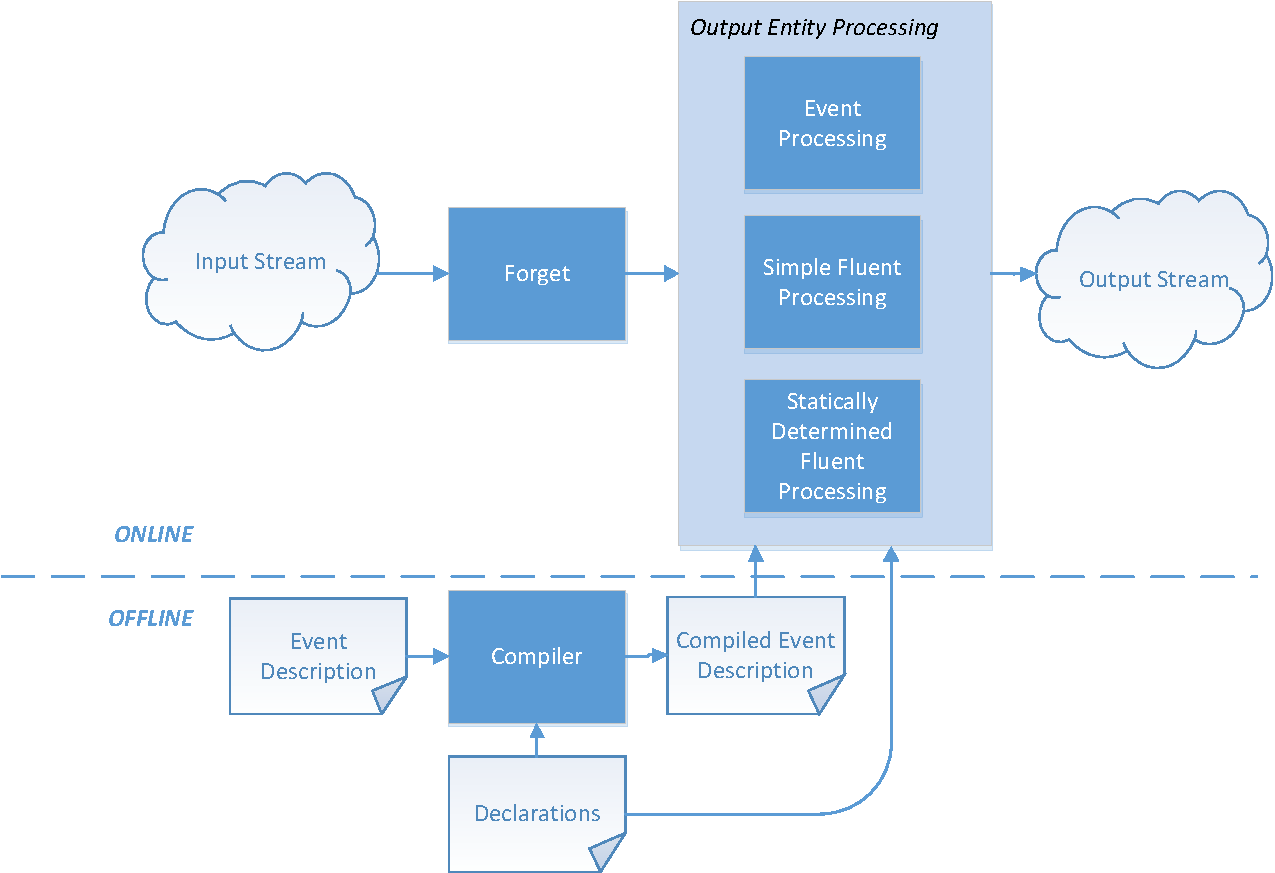
\includegraphics[width=0.8\textwidth]{figures/RTEC_diagram}}
	\caption{The architecture of RTEC.}
	\label{fig:rtec-main}
\end{figure}

\subsection{Offline Activities}\label{sec:compilation}

Before the commencement of online activities, RTEC compiles the event description into a format that allows for more efficient reasoning. This is an offline process which is transparent to the user. 
%
The compiler is called via the predicate: 

{\small
\begin{verbatim}
   ?- compileEventDescription(+Declarations, +EventDecription, 
                              -CompiledEventDescription).
\end{verbatim}
}

The input of this predicate is the event description file (such as Listing \ref{lst:rules}) and the declarations file (e.g.~Listing \ref{lst:declarations}). The output of this predicate is the compiled event description file which is subsequently used for online reasoning --- see the bottom part (`offline') of Figure \ref{fig:rtec-main}.

The aim of the compilation is to eliminate the number of unsuccessful evaluations of \happensAt, \holdsFor\ and \holdsAt, and to introduce additional indexing information.
These atoms are rewritten using specialised predicates, depending on whether they appear in the head or the body of a rule, whether they concern a simple or a statically determined fluent, and whether they host an input or an output entity.

When a \happensAt\ predicate appears in the head of a rule in the Event Description, it is converted into \happensAtEv. On the other hand, \happensAt\ predicates that appear in the body of a rule are converted into \happensAtIE\ (for events that are input entities) or \happensAtProcessed\ (for events that are output entities).

Similarly, the \holdsFor\ predicates appearing in the head of a domain-dependent rule, i.e.~a rule for computing the maximal intervals of statically determined fluents, are rewritten using the predicate \holdsForSDFluent. \holdsFor\ predicates appearing in the body of a rule are translated into \holdsForProcessedSimpleFluent, \holdsForProcessedIE\ or \holdsForProcessedSDFluent\ predicates, according to the fluent type they concern: simple fluents, input (statically determined) fluents, and output statically determined fluents, respectively.

In contrast to the \happensAt\ and \holdsFor\ predicates, \holdsAt\ does not appear in the head of a rule. However, it may appear in the body of \initiatedAt\ and \terminatedAt\ rules; in the case of a simple fluent, the body \holdsAt\ predicate is converted to a \holdsAtProcessedSimpleFluent, whereas in the case of input or output statically determined fluent, it is converted into a \holdsAtProcessedIE\ or a \holdsAtProcessedSDFluent, respectively.

\begin{comment}
\begin{algorithm}[h]                   
\caption{\textttsmall{rtec(}$\mathit{Q_i,\ \omega}$\textttsmall{)} $\qquad\qquad\qquad\qquad\qquad\qquad\qquad\qquad\qquad\qquad\qquad\qquad\qquad\qquad\quad$   
{\small \textbf{Input: }\textttsmall{k}: Depth of hierarchical event description;\ \textttsmall{SimpleFluents(n)}: simple fluents of level \textttsmall{n}; \textttsmall{StdFluents(n)}: statically determined fluents of level \textttsmall{n};\ \textttsmall{Events(n)}: events of level \textttsmall{n}} }
\label{pc:main-RTEC}                          
\begin{algorithmic}[1]
\STATE \textttsmall{forget}$\mathit{( Q_i{-}\omega )}$
%\STATE cachingOrder2(Index,OE)
%\STATE (
%\STATE 
\FOR{\textttsmall{n:=1; n=<k; n++}}
\FORALL{\textttsmall{Std} $\in$ \textttsmall{StdFluents(n)}}  
  \STATE \textttsmall{processSDFluent(Std, }$\mathit{Q_i{-}\omega}$\textttsmall{)}
\ENDFOR
\FORALL{\textttsmall{Se} $\in$ \textttsmall{SimpleFluents(n)}}  
  \STATE \textttsmall{processSimpleFluent(Se, }$\mathit{Q_i{-}\omega}$\textttsmall{)}
\ENDFOR
\FORALL{\textttsmall{Ev} $\in$ \textttsmall{Events(n)}} %\textbf{then} 
  \STATE \textttsmall{processEvent(Ev, }$\mathit{Q_i{-}\omega}$\textttsmall{)}
\ENDFOR
\ENDFOR
\end{algorithmic}
\end{algorithm}
\end{comment}

\subsection{Online Activities}

%Algorithm \ref{pc:main-RTEC} shows the pseudo-code of the main loop of RTEC. 
As already mentioned, reasoning is performed by means of continuous query processing, and concerns the computation of the maximal intervals of output entities, i.e.~the intervals of simple and statically determined fluents, as well as the time-points in which events occur. At each query time $Q_i$, all input entities that took place before or at $Q_i{-}\omega$ are discarded/`forgotten' (see the `forget' box in Figure \ref{fig:rtec-main}).  
Then, RTEC computes and stores the intervals of each output entity (see `output entity processing' in Figure \ref{fig:rtec-main}). Recall that attention is restricted to hierarchical event descriptions. The form of the hierarchy is specified by the event description developer in the declarations using the \textttsmall{cachingOrder} predicate (see Section \ref{sec:declarations}).
%
RTEC adopts a caching technique where the fluents and events of the event description are processed in a bottom-up manner; this way, the intervals (resp.~time-points) of the fluents (events) that are required for the processing of a fluent (event) of level $n$ will simply be fetched from the cache without the need for re-computation. %This technique is illustrated in the outer for-loop of Algorithm \ref{pc:main-RTEC} (see lines 2--12) where fluent (event) processing starts at level 1 of the hierarchical event description and proceeds towards the top (\textttsmall{k}) level. %The fluents (events) of the same level may be processed in any order. For illustration purposes, in Algorithm 1 the following order is adopted: statically determined fluents (lines 4--6), simple fluents (lines 7--9) and events (lines 10--12).
In the following sections we discuss the processes of `forgetting', fluent and event processing. 

\subsubsection{Forget Mechanism}

At each query time $Q_i$, RTEC first discards --- `forgets' --- all input entities that end before or on $\mathit{Q_i{-}\omega}$. For each input entity available at $Q_i$, RTEC:
%
\begin{itemize}
 \item Completely retracts the input entity if the interval attached to it ends before or on $\mathit{Q_i{-}WM}$.
 \item Partly retracts the interval of the input entity if it starts before or on $\mathit{Q_i{-}WM}$ and ends after that time. More precisely, RTEC retracts the input entity interval \textttsmall{(Start,End)} and asserts the interval \textttsmall{(}$\mathit{Q_i{-}\omega}$\textttsmall{,End)}. 
\end{itemize}   

\subsubsection{Statically Determined Fluent Processing}

%The next operation is about looking for intervals in which output Statically Determined Fluents hold. The \textttsmall{processSDFluents} operation follows the same approach as the previous two operations. This time we are looking for \textttsmall{holdsForSDFluent} predicates in the compiled Event description file. In this case, \textttsmall{processSDFluents} will construct this interval from the intervals of the Fluents in the body of the \textttsmall{holdsForSDFluent} clause. To do this, our operation uses ``Interval manipulation'' techniques, in the auxiliary ``Utilities'' module.

After `forgetting' input entities, RTEC computes and stores the intervals of each output entity. At the end of reasoning at each query time $Q_i$, all computed fluent intervals are stored in the computer memory as \simpleFPList\ and \sdFPList\ assertions. \textttsmall{I} in \textttsmall{sdFPList(Index, std, I, PE)} (resp.~\textttsmall{simpleFPList(Index, se, I, PE)}) represents the intervals of statically determined fluent \textttsmall{Std} (simple fluent \textttsmall{Se}) starting in $(Q_{i}{-}\omega, Q_{i}]$, sorted in temporal order. \textttsmall{PE} stores the interval, if any, ending at $Q_{i}{-}\omega$. The first argument in \sdFPList\ (\simpleFPList) is an index that allows for the fast retrieval of stored intervals for a given fluent  even in the presence of very large numbers of fluents. When the user queries  the maximal intervals of a fluent, RTEC amalgamates \textttsmall{PE} with the intervals in \textttsmall{I}, producing a list of maximal intervals ending in $[Q_{i}{-}\omega, Q_{i}]$ and, possibly, an open interval starting in $[Q_{i}{-}\omega, Q_{i}]$.


\begin{algorithm}[h]                   
\caption{ \textttsmall{processSDFluent(Std,}\ $\mathit{Q_i{-}\omega}$\textttsmall{)} }  
\label{pc:recogniseSDFluent}                          
\begin{algorithmic}[1]
\STATE \textttsmall{indexOf(Std, Index)}
\STATE \textttsmall{retract(sdFPList(Index, Std, OldI, OldPE))}
\STATE \textttsmall{amalgamate(OldPE, OldI, OldList)}
\IF {\textttsmall{Start,End:[Start,End)} $\in$ \textttsmall{OldList } $\wedge\ $ \textttsmall{End>}$\mathit{Q_i{-}\omega\ \wedge\ }$ \textttsmall{Start=<} $\mathit{Q_i{-}\omega}$ } %\textbf{then} 
\STATE \textttsmall{PE:=[(Start,}$\mathit{Q_i{-}\omega{+}1}$\textttsmall{)]}
\ELSE 
\STATE \textttsmall{PE:=[]}
\ENDIF 
\STATE \textttsmall{holdsFor(SF, I)}
\STATE \textttsmall{assert(sdFPList(Index, SF, I, PE))}
\end{algorithmic}
\end{algorithm}


Listing \ref{pc:recogniseSDFluent} shows the pseudo-code of \processSDFluent, the procedure for computing and storing the intervals of statically determined fluents. First, RTEC retrieves from \sdFPList\ the maximal intervals of a statically determined fluent \textttsmall{Std} computed at $Q_{i{-}1}$ and checks if there is such an interval that overlaps $Q_i{-}\omega$ (lines 1--8). In Listing~\ref{pc:recogniseSDFluent}, \textttsmall{OldI} represents the intervals of \textttsmall{Std} computed at $Q_{i-1}$. These intervals are temporally sorted and start in $(Q_{i-1}{-}\omega, Q_{i-1}]$. \textttsmall{OldPE} stores the interval, if any, ending at $Q_{i-1}{-}\omega$. RTEC amalgamates \textttsmall{OldPE} with the intervals in \textttsmall{OldI}, producing \textttsmall{OldList} (line 3). If there is an interval  $[$\textttsmall{Start,End}$)$ in \textttsmall{OldList} that overlaps $Q_i{-}\omega$, then the sub-interval $[$\textttsmall{Start,}$\mathit{Q_i{-}\omega{+}1)}$ is retained. See \textttsmall{PE} in Listing \ref{pc:recogniseSDFluent}. All intervals in \textttsmall{OldList} after $Q_i{-}\omega$ are discarded.

At the second step of \processSDFluent, RTEC evaluates \holdsForSDFluent\ rules to compute the \textttsmall{Std} intervals from input entities recorded as occurring in $(Q_i{-}\omega, Q_i]$ (line 9). Prior to the run-time recognition process, RTEC has transformed \holdsFor\ rules concerning statically determined fluents into \holdsForSDFluent\ rules, in order to avoid unnecessary \holdsFor\ rule evaluations (see Section \ref{sec:compilation} for the compilation stage). The intervals of \textttsmall{Std} computed at the previous query time $Q_{i-1}$ are not taken into consideration in the evaluation of \holdsForSDFluent\ rules. The computed list of intervals \textttsmall{I} of \textttsmall{Std}, along with \textttsmall{PE}, are stored in \sdFPList\ (line 10), replacing the intervals computed at $Q_{i-1}$. (Recall that, when the user queries the maximal intervals of a fluent, RTEC amalgamates \textttsmall{PE} with the intervals in \textttsmall{I}.)



\subsubsection{Simple Fluent Processing}

\processSimpleFluent, the procedure for computing and storing simple fluent intervals, also has two parts. First, RTEC checks if there is a maximal interval of the fluent \textttsmall{Se} that overlaps $Q_i{-}\omega$. If there is such an interval then it will be discarded, while its starting point will be kept. 
Second, RTEC computes the starting points of \textttsmall{Se} by evaluating \initiatedAt\ rules, without considering the starting points calculated at $Q_{i-1}$. The starting points are given to \holdsForSimpleFluent, into which \holdsFor\ calls computing the maximal intervals of simple fluents are translated at compile time. This program is defined as follows:

{\small
\begin{verbatim}
holdsForSimpleFluent(SP, Se, I) :- 
     SP <> [],
     computeEndingPoints(Se, EP),
     makeintervals(SP, EP, I).
\end{verbatim}
}

If the list of starting points is empty (first argument of \holdsForSimpleFluent) then the empty list of intervals is returned. Otherwise, \holdsForSimpleFluent\ computes the ending points \textttsmall{EP} of the fluent by evaluating \terminatedAt\ rules, without considering the ending points calculated at $Q_{i-1}$, and then uses \textttsmall{makeIntervals} to compute its maximal intervals given its starting and ending points. 

\begin{figure}[h]
    \centering
    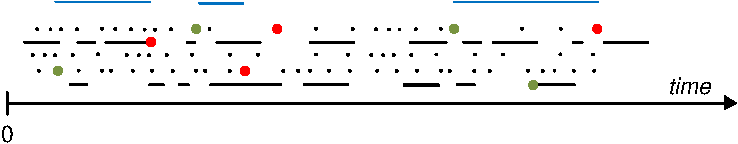
\includegraphics[width=.6\textwidth]{figures/sf4}
    \caption{Maximal interval computation for simple fluents.}
    \label{fig:makeIntervals}
\end{figure}

Figure \ref{fig:makeIntervals} illustrates the process of \textttsmall{makeIntervals}. The black lines and dots indicate streams of durative and instantaneous input entities. The green dots denote starting/initiating points while the red dots indicate ending/terminating points.  
Note that \textttsmall{initiatedAt(F=V, T)} does not necessarily imply that \textttsmall{F<>V} at \textttsmall{T}. Similarly, \textttsmall{terminatedAt(F=V, T)} does not necessarily imply that \textttsmall{F=V} at \textttsmall{T}. 
\textttsmall{makeIntervals} finds all time-points \textttsmall{Ts} at which the fluent \textttsmall{Se} is initiated, and then, for each \textttsmall{Ts}, it computes the first time-point \textttsmall{Tf} after \textttsmall{Ts} at which \textttsmall{Se} is terminated.
Suppose, for example, that  \textttsmall{Se} is initiated at time-points 10 and 20 and terminated at time-points 25 and  30 (and at no other time-points). In that case \textttsmall{Se} holds at all \textttsmall{T} such that 10 $<$ \textttsmall{T} $\leq$ 25. 

\subsubsection{Event Processing}

\textttsmall{processEvents} is the procedure for computing and storing the time-points in which output events occur. In brief, \textttsmall{processEvents} first retracts all computed time-points of the output event in $(Q_{i}-\omega, Q_i]$, and then evaluates \textttsmall{happensAtEv} rules into which domain-dependent \happensAt\ calls are translated at compile time.